\section{Sobol采样器}\label{sec:Sobol采样器}
\begin{remark}
    本节含有高级内容,第一次阅读时可以跳过。
\end{remark}

本章最后一个\refvar{Sampler}{}基于Sobol确定的一系列生成矩阵。
来自这些矩阵生成的序列的样本的区别在于能非常高效地实现——
因为是完全基于2进制计算的——而且在样本向量的全部$n$个维度上都分布得极好。
\reffig{7.34}展示了前几个Sobol生成矩阵。
\begin{figure}[htbp]
    \centering
    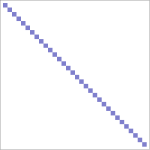
\includegraphics[width=0.24\linewidth]{chap07/sobol0.png}\,
    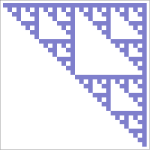
\includegraphics[width=0.24\linewidth]{chap07/sobol1.png}\,
    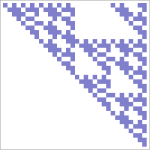
\includegraphics[width=0.24\linewidth]{chap07/sobol2.png}\,
    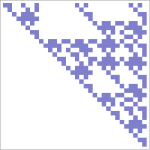
\includegraphics[width=0.24\linewidth]{chap07/sobol3.png}
    \caption{Sobol序列前四维的生成矩阵。注意其规则的结构。}
    \label{fig:7.34}
\end{figure}

\reffig{7.35}用景深测试场景比较了Sobol样本以及分层和Halton点。
\begin{figure}[htbp]
    \subfloat[分层采样]{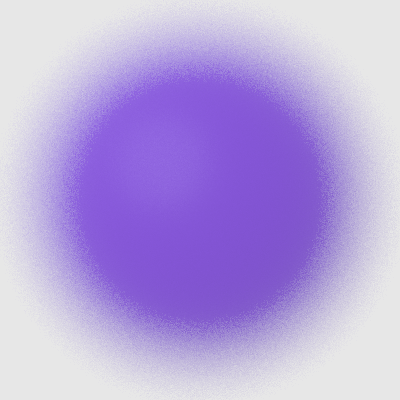
\includegraphics[width=0.49\linewidth]{chap07/dof-stratified.png}\label{fig:7.35.1}}\,
    \subfloat[Halton采样]{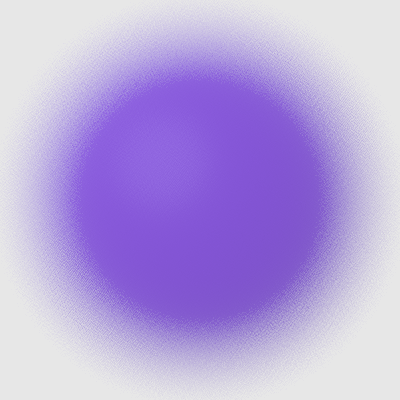
\includegraphics[width=0.49\linewidth]{chap07/dof-halton.png}\label{fig:7.35.2}}\\
    \subfloat[Sobol采样]{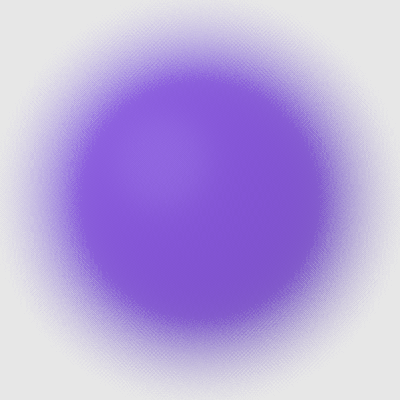
\includegraphics[width=0.49\linewidth]{chap07/dof-sobol.png}\label{fig:7.35.3}}
    \caption{为渲染景深比较分层、Halton以及Sobol采样器。
        (a)用\refvar{StratifiedSampler}{}渲染的图像,
        (b)用\refvar{HaltonSampler}{}渲染的图像,以及
        (c)用\refvar{SobolSampler}{}渲染的图像。
        两个低偏差采样器都比分层采样器要好。尽管使用\refvar{SobolSampler}{}的该欠采样图像
        能看到结构化的网格伪影,但Sobol序列经常提供比Halton序列更快的收敛速度。}
    \label{fig:7.35}
\end{figure}

Sobol点的缺点是它们在收敛前容易出现结构化网格伪影;
在\reffig{7.36}展示的图像样本点中可以看出该问题。
\begin{figure}[htbp]
    \centering\includegraphics[width=0.5\linewidth]{chap07/sobol2x2pix.eps}
    \caption{$2\times2$像素的网格,每个用16个Sobol样本采样。
        注意有大量结构,且许多样本互相靠近。该序列在样本向量全部$n$个维度上
        极好的分布性质通常弥补了这些缺点。}
    \label{fig:7.36}
\end{figure}

在\reffig{7.37}的图像中该结构是可见的。
该缺点换来的是,Sobol序列在样本序列全部$n$个维度上分布得极其好。
\begin{figure}[htbp]
    \centering
    \subfloat[Halton采样器]{\includegraphics[width=\linewidth]{chap07/car-halton-undersampled.png}\label{fig:7.37.1}}\\
    \subfloat[Sobol采样器]{\includegraphics[width=\linewidth]{chap07/car-sobol-undersampled.png}\label{fig:7.37.2}}
    \caption{用(a)Halton采样器和(b)Sobol采样器渲染的欠采样图像。
        虽然具有不同的视觉特征,但两个都展现出可见的结构。
        特别是Sobol序列展现出清晰可见的棋盘结构。}
    \label{fig:7.37}
\end{figure}

\begin{lstlisting}
`\initcode{SobolSampler Declarations}{=}`
class `\initvar{SobolSampler}{}` : public `\refvar{GlobalSampler}{}` {
public:
    `\refcode{SobolSampler Public Methods}{}`
private:
    `\refcode{SobolSampler Private Data}{}`
};
\end{lstlisting}

\refvar{SobolSampler}{}用能让样本域$[0,1)^2$覆盖住要采样的图像区域
的最小幂2值来均匀缩放前两维。像\refvar{HaltonSampler}{}那样,
选择该特定缩放方案是为了更容易计算从像素坐标到每个像素内样本索引的逆映射。
\begin{lstlisting}
`\initcode{SobolSampler Public Methods}{=}`
`\refvar{SobolSampler}{}`(int64_t samplesPerPixel, const `\refvar{Bounds2i}{}` &sampleBounds)
    : `\refvar{GlobalSampler}{}`(`\refvar{RoundUpPow2}{}`(samplesPerPixel)),
      `\refvar{sampleBounds}{}`(sampleBounds) {
    `\refvar{resolution}{}` = `\refvar{RoundUpPow2}{}`(std::max(sampleBounds.`\refvar{Diagonal}{}`().x,
                                      sampleBounds.`\refvar{Diagonal}{}`().y));
    `\refvar{log2Resolution}{}` = `\refvar{Log2Int}{}`(`\refvar{resolution}{}`);
}
\end{lstlisting}
\begin{lstlisting}
`\initcode{SobolSampler Private Data}{=}`
const `\refvar{Bounds2i}{}` `\initvar{sampleBounds}{}`;
int `\initvar{resolution}{}`, `\initvar{log2Resolution}{}`;
\end{lstlisting}

如果采样域$[0,1)^2$已被缩放$2^{\text{\refvar{log2Resolution}{}}}$倍
以覆盖像素采样区域,则函数\refvar{SobolIntervalToIndex}{()}返回
像素{\ttfamily p}内第{\ttfamily sampleNum}个样本的索引。
\begin{lstlisting}
`\refcode{Low Discrepancy Declarations}{+=}\lastcode{LowDiscrepancyDeclarations}`
inline uint64_t `\initvar{SobolIntervalToIndex}{}`(const uint32_t log2Resolution,
    uint64_t sampleNum, const `\refvar{Point2i}{}` &p);
\end{lstlisting}

用于推导它所实现的算法的一般方法和Halton采样器在其方法\linebreak
\refvar[HaltonSampler::GetIndexForSample]{GetIndexForSample}{()}中用的一样。
积${\bm C}[d_i(a)]^{\mathrm{T}}$构建了缩放后样本的整数部分,
这里用幂2缩放意味着缩放值以2为底的对数给出了它的位数。
为了求得缩放后能给出特定整数值的$a$值,我们可以计算$\bm C$的逆:设
\begin{align*}
    v={\bm C}[d_i(a)]^{\mathrm{T}}\, ,
\end{align*}
则等价地
\begin{align*}
    {\bm C}^{-1}v=[d_i(a)]^{\mathrm{T}}\, .
\end{align*}
我们这里不会介绍该方法的实现。
\begin{lstlisting}
`\initcode{SobolSampler Method Definitions}{=}\initnext{SobolSamplerMethodDefinitions}`
int64_t `\refvar{SobolSampler}{}`::`\initvar[SobolSampler::GetIndexForSample]{\refvar{GetIndexForSample}{}}{}`(int64_t sampleNum) const {
    return `\refvar{SobolIntervalToIndex}{}`(`\refvar{log2Resolution}{}`, sampleNum,
        `\refvar{Point2i}{}`(`\refvar{currentPixel}{}` - `\refvar{sampleBounds}{}`.`\refvar{pMin}{}`));
}
\end{lstlisting}

有了函数\refvar{SobolSample}{()},为给定样本索引和维度计算样本值很简单。
\begin{lstlisting}
`\refcode{SobolSampler Method Definitions}{+=}\lastcode{SobolSamplerMethodDefinitions}`
`\refvar{Float}{}` `\refvar{SobolSampler}{}`::`\initvar[SobolSampler::SampleDimension]{\refvar{SampleDimension}{}}{}`(int64_t index, int dim) const {
    `\refvar{Float}{}` s = `\refvar{SobolSample}{}`(index, dim);
    `\refcode{Remap Sobol dimensions used for pixel samples}{}`
    return s;
}
\end{lstlisting}

计算Sobol样本值的代码对32和64位浮点值采用不同的路径。
两种情况使用不同的生成矩阵,为64位双精度给出更多精度位数。
\begin{lstlisting}
`\refcode{Low Discrepancy Inline Functions}{+=}\lastnext{LowDiscrepancyInlineFunctions}`
inline `\refvar{Float}{}` `\initvar{SobolSample}{}`(int64_t index, int dimension,
                         uint64_t scramble = 0) {
#ifdef PBRT_FLOAT_AS_DOUBLE
    return `\refvar{SobolSampleDouble}{}`(index, dimension, scramble);
#else
    return `\refvar{SobolSampleFloat}{}`(index, dimension, scramble);
#endif
}
\end{lstlisting}

函数\refvar{SobolSampleFloat}{()}的实现和\refvar{MultiplyGenerator}{()}非常像,
区别是它接收64位索引,所用的矩阵尺寸是$32\times52$.
这些更大的矩阵允许它生成不同的样本值至$a=2^{52}-1$,
而不是之前所用$32\times32$矩阵的$2^{32}-1$.
\begin{lstlisting}
`\refcode{Low Discrepancy Inline Functions}{+=}\lastcode{LowDiscrepancyInlineFunctions}`
inline float `\initvar{SobolSampleFloat}{}`(int64_t a, int dimension,
                              uint32_t scramble) {
    uint32_t v = scramble;
    for (int i = dimension * `\refvar{SobolMatrixSize}{}`; a != 0; a >>= 1, ++i)
        if (a & 1)
            v ^= `\refvar{SobolMatrices32}{}`[i];
    return v * 0x1p-32f; /* 1/2^32 */
}
\end{lstlisting}
\begin{lstlisting}
`\initcode{Sobol Matrix Declarations}{=}`
static constexpr int `\initvar{NumSobolDimensions}{}` = 1024;
static constexpr int `\initvar{SobolMatrixSize}{}` = 52;
extern const uint32_t `\initvar{SobolMatrices32}{}`[`\refvar{NumSobolDimensions}{}` *
                                      `\refvar{SobolMatrixSize}{}`];
\end{lstlisting}

函数{\initvar{SobolSampleDouble}{()}}类似,除了它用64位的Sobol矩阵。
这里没有在文中介绍它。

因为\refvar{SobolSampler}{}是种\refvar{GlobalSampler}{},
所以为前两维返回的值需要被调整使其变为对当前像素的偏移量。
这里用构造函数算出的幂2系数放大样本值,再对样本框的左下角
\sidenote{译者注:原文lower corner,确切翻译的话指坐标值最小的角点。}偏移
以求得对应的栅格样本位置。减去当前整数像素坐标就得到$[0,1)$内的结果。
\begin{lstlisting}
`\initcode{Remap Sobol dimensions used for pixel samples}{=}`
if (dim == 0 || dim == 1)  {
    s = s * `\refvar{resolution}{}` + `\refvar{sampleBounds}{}`.`\refvar{pMin}{}`[dim];
    s = `\refvar{Clamp}{}`(s - `\refvar{currentPixel}{}`[dim], (`\refvar{Float}{}`)0, `\refvar{OneMinusEpsilon}{}`);
}
\end{lstlisting}